\section{Исходные данные}
\addcontentsline{toc}{section}{Исходные данные}	% Добавляем его в оглавление

\begin{figure}[h!t]
  		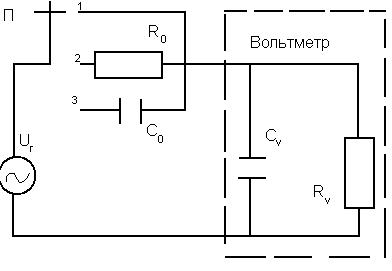
\includegraphics[width=0.25\linewidth]{scheme1}
  		\centering{\caption{Схема электронного ключа}}
\end{figure}

\begin{multicols}{3}

\text{транзистор VT-KT315Б}

$ R_{\text{Г}} = $ 4,7 кОм

$ R_{\text{Б}} = $ 4,7 кОм

$ R_{\text{К}} = $ 2,2 кОм

$ R_{\text{н}} = \infty $

$ C_{\text{н}} = $ 0 

$ U_{\text{ИП}} = $ 10 В

$ U_{\text{СМ}} = $ -4 В

\end{multicols}
